

\groupphoto{0.93}{0.8}{./chap/1900-1925/MGH-1905.jpg}
{\emph{Erstes Vereinsfoto 1905}\\
    Von links nach rechts sitzend:\\
    Estermann Josef, Halden, Troxler Xaver, Wiederkehr, Muff Peter, Lehrer,
    Troxler Kaspar, Moos\\
    Von links nach rechts stehend:\\
    Bühlmann Rudolf, Hermetsmatt, Müller Heinrich, Dorf, Estermann Heinrich,
    Traselingen, Suter Kaspar, Dorf, Suter Hans-Georg, Dorf} {fig:mgh-1905}

\begin{history}

    % \subsection{1900-1925}

    Wenn auch diese Zeitspanne Mitgliederwechsel brachte, so konnte doch ein
    langsames Wachsen und Gedeihen der Musikgesellschaft festgestellt werden.
    Ihre Mitgliederzahl erhöhte sich von zehn auf neunzehn Mann. Die Tätigkeit
    bestand in den ersten Jahren noch vorwiegend aus dem Musizieren bei
    Ständchen, Ausmärschen und Tanzanlässen.

    Dass die Musikgesellschaft Hildisrieden bemüht war, gute Beziehungen zu
    Kirchenchor und Schützengesellschaft zu pflegen, beweisen die gemeinsamen
    Konzerte und Ausflüge auf die Rigi, nach Engelberg und Andermatt. Die Musik
    betrachtete ihre Aufgabe aber nicht bloss im Tanzmusikspielen, Sie war
    jederzeit bereit aufzutreten, wenn sich irgendetwas tat in der Gemeinde. Das
    zeigte die Einweihungsfeier unserer neuen Kirche im Jahre 1904. Der Verein
    war bestrebt, diesem Anlass ein festliches Gepräge zu geben und erfreute mit
    seinen Beiträgen den Bischof Leonard Haas und all die vielen Gäste.

    Im Verlaufe des Herbstes gleichen Jahres wurde die Gesellschaft zur
    Unterhaltung zu einem Grossanlass nach Münster aufgeboten. Es ging um das
    umstrittene Wynentalbahn-Projekt, das damals viel Gesprächsstoff lieferte,
    hätte doch die Weiterführung der Linie über Hildisrieden bis Emmenbrücke
    unser Dorf in der Entwicklung beeinflusst. (Geplanter Bahnhof bei der
    heutigen Bäckerei Arnold).

    Die Musikgesellschaft wurde 1905 erstmals photografiert.

    Dass der Probenbesuch nicht immer den Wünschen des Kapellmeisters entsprach,
    zeigt das Probenverzeichnis von 1907. Von den 15 abgehaltenen Proben trug
    nur eine den Vermerk \enquote{Alle anwesend}. Stets war die Musik bereit,
    ihren Möglichkeiten entsprechend mitzuwirken, so 1909 am Pfarraufritte von
    Pfarrer Alois Hodel.

    In den Jahren 1910 und 1911 sind nebst den kirchlichen und den weltlichen
    Anlässen keine weiteren Taten zu verzeichnen, ebenso schweigt das
    Probenverzeichnis.

    An der Generalversammlung vom 31. März 1912 wurden die Statuten wieder
    revidiert und von folgenden Mitgliedern unterzeichnet:

    \noindent
    Karl Estermann, Traselingen\\
    Peter Muff, Lehrer\\
    Alois Estermann, Traselingen\\
    Kaspar Troxler, Moos\\
    Kaspar Suter, Dorf\\
    Alois Troxler, Schopfen\\
    Franz Troxler, Schopfen\\
    Josef Troxler, Schopfen\\
    Alois Wolf, Sandgütsch\\
    Josef Gassmann, Gigen\\
    Balz Gassmann, Gigen\\
    Heinrich Estermann, Dorf

    Der Rechnungsbericht, abgelegt von Kassier Kaspar Troxler, verzeigte an
    Einnahmen Fr. 298.90 und an Ausgaben Fr. 79.22. Die Mehreinnahmen wurden
    verteilt, und jedes Mitglied konnte 15 Franken als \enquote{Dividende}
    entgegennehmen.

    Dass die Musikgesellschaft 1915 neue Mitglieder aufnehmen konnte, bezeugt,
    dass der Verein bestrebt war, sich weiterzuentwickeln und an sich zu
    arbeiten. Neu wurden in den Verein aufgenommen: Josef Disler, Dorf; Jakob
    Estermann, Bethlehem; Heinrich Estermann, Ohmenlingen; Heinrich Estermann,
    Dorf; Josef Jutz, Löwen, und Leo Erni, Schmiede.

    Diese Mitglieder haben das Vereinsschifflein in gesellschaftlicher Hinsicht
    wieder belebt und flotte Probenarbeit geleistet. Die Musikgesellschaft hatte
    sich nun schon derart gefestigt, dass der entfachte Weltkrieg das
    Vereinsleben nicht mehr zum Stillstand zu bringen vermochte. Bei jeder, wenn
    auch nur selten sich bietenden Gelegenheit, wurden Proben abgehalten.

    Im Jahre 1915 hatte der Vorstand folgendes Aussehen:

    \noindent
    Präsident: Kaspar Suter, Dorf\\
    Dirigent Alois Estermann, Traselingen\\
    Aktuar: Karl Estermann, Traselingen\\
    Kassier: Kaspar Troxler, Moos\\
    Mitglied: Alois Troxler, Lenzenhof

    \enquote{Friede ist es zwar geworden, das Elend und der Hass unter den
        Völkern ist geblieben}, so beginnt der Tätigkeitsbericht von 1919,
    Arbeitslosigkeit und Unzufriedenheit herrschten in der Heimat. Als in
    den ersten Augusttagen das tapfere Inf Reg 19 nach Zürich gerufen wurde,
    um Ruhe und Ordnung zu schaffen, betraf das auch Hildisrieder
    Musikanten,

    Am Jubiläumsschiessen der Schützengesellschaft Hildisrieden gab die Musik im
    Löwen ein Konzert zum besten.

    Das Symbol des Vereins, die Fahne, die 40 Jahre Wind und Wetter getrotzt
    hatte, sollte ersetzt werden. Eine von Frauen und Töchtern Hildisriedens im
    Frühjahr 1921 durchgeführte Sammlung, ermöglichte dieses Vorhaben. Besondere
    Aufmerksamkeit schenkte man der Musikgesellschaft bei der Teilnahme am
    Kantonalen Musiktag in Sempach unter der Leitung von Lehrer Alois Troxler.

    An der Gemeindeversammlung vom 25. März 1924 beantragte Josef Disler sen.,
    dass der jährliche Beitrag der Gemeinde von Fr. 40.— auf Fr. 100,— erhöht
    werden sollte, was auch einstimmig genehmigt wurde. Von nun an wurde
    intensiver und freudiger musiziert.

    \subsubsection{Zweite Fahnenweihe 1921}

    Nachdem im Verlaufe der Generalversammlung vom 29. Mai 1921 der Wunsch nach
    einer neuen Fahne laut wurde, erhielt der Präsident Kaspar Suter den
    Auftrag, diese Angelegenheit nun ernsthaft an die Hand zu nehmen. Man war
    sich einig, dass die 40-jährige Fahne, die Wind und Wetter getrotzt hat,
    ersetzt werden sollte. Die nötige Geldsammlung wurde von acht Töchtern
    besorgt. Frl. Rosa Estermann, Grossrats, Ohmenlingen, stand als Präsidentin
    an der Spitze. Der abgelieferte Betrag von Fr. 1024.— übertraf alle
    Erwartungen und wurde dankbar entgegengenommen.\\
    \\
    Fahnenweihe vom 4. September 1921\\
    Mittags 14 Uhr Festzug vom Schulhaus zur Kirche; Josef Estermann, Halden,
    marschierte als Fähnrich mit verhüllter Fahne, umgeben von Ehrendamen,
    Patenpaars und Gästen in die Kirche. Im Chor wurde das Banner entrollt und
    vom Ortspfarrer Alois Hodel eingesegnet. Des schlechten Wetters wegen fand
    die Übergabe im Löwensaal statt. Voller Freude überreichten Heinrich
    Estermann, Ohmenlingen, als Götti und Elisabeth Zwinggi, von Schopfen, als
    Gotte ihren Musikfreunden das recht hübsch präsentierende Banner.

    Es trägt die Inschrift :\enquote{In Freud und Leid zum Spiel bereit}.

\end{history}


\begin{figure}[ht]
    \subfloat[Dorfplatz mit Vierwaldstätterhof]{%
        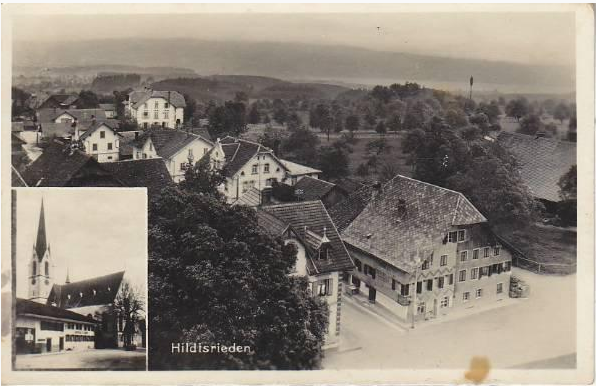
\includegraphics[height=0.5\textheight,keepaspectratio]{./Dorf-Bilder/p18}
    }\hfil
    \subfloat[Um 1920]{%
        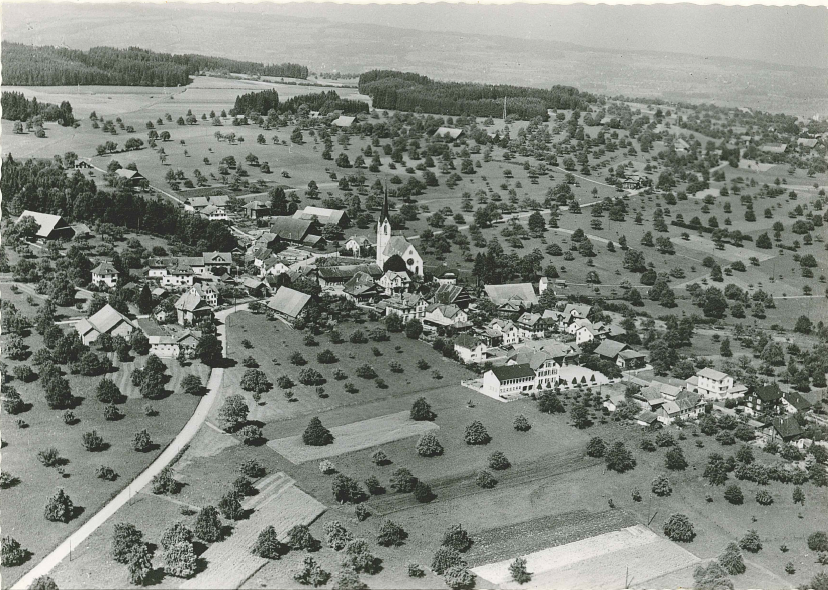
\includegraphics[height=0.5\textheight,keepaspectratio]{./Dorf-Bilder/p12}
    }
\end{figure}

\clearpage

\groupphoto{0.93}{0.8}{./chap/1900-1925/MGH-1921.jpg}
{ \emph{Die Musikgesellschaft 1921}\\
    Von links nach rechts sitzend:\\
    Estermann Heinrich, Troxler Kaspar, Troxler Alois, Dirigent, Estermann Alois,
    Troxler Alois\\
    1. Reihe stehend:\\
    Disler Josef, Estermann Heinrich, Suppiger Hans, Estermann Jakob, Zwinggi
    Josef, Suter Josef, Erni Leo, Zwinggi Jakob, Suter Kaspar, Gassmann Balz\\
    2. Reihe stehend:\\
    Estermann Karl, Estermann Josef, Estermann Jakob, Estermann
    Jakob}{fig:mgh-1921}

\begin{figure}[!ht]
    \centerline{
        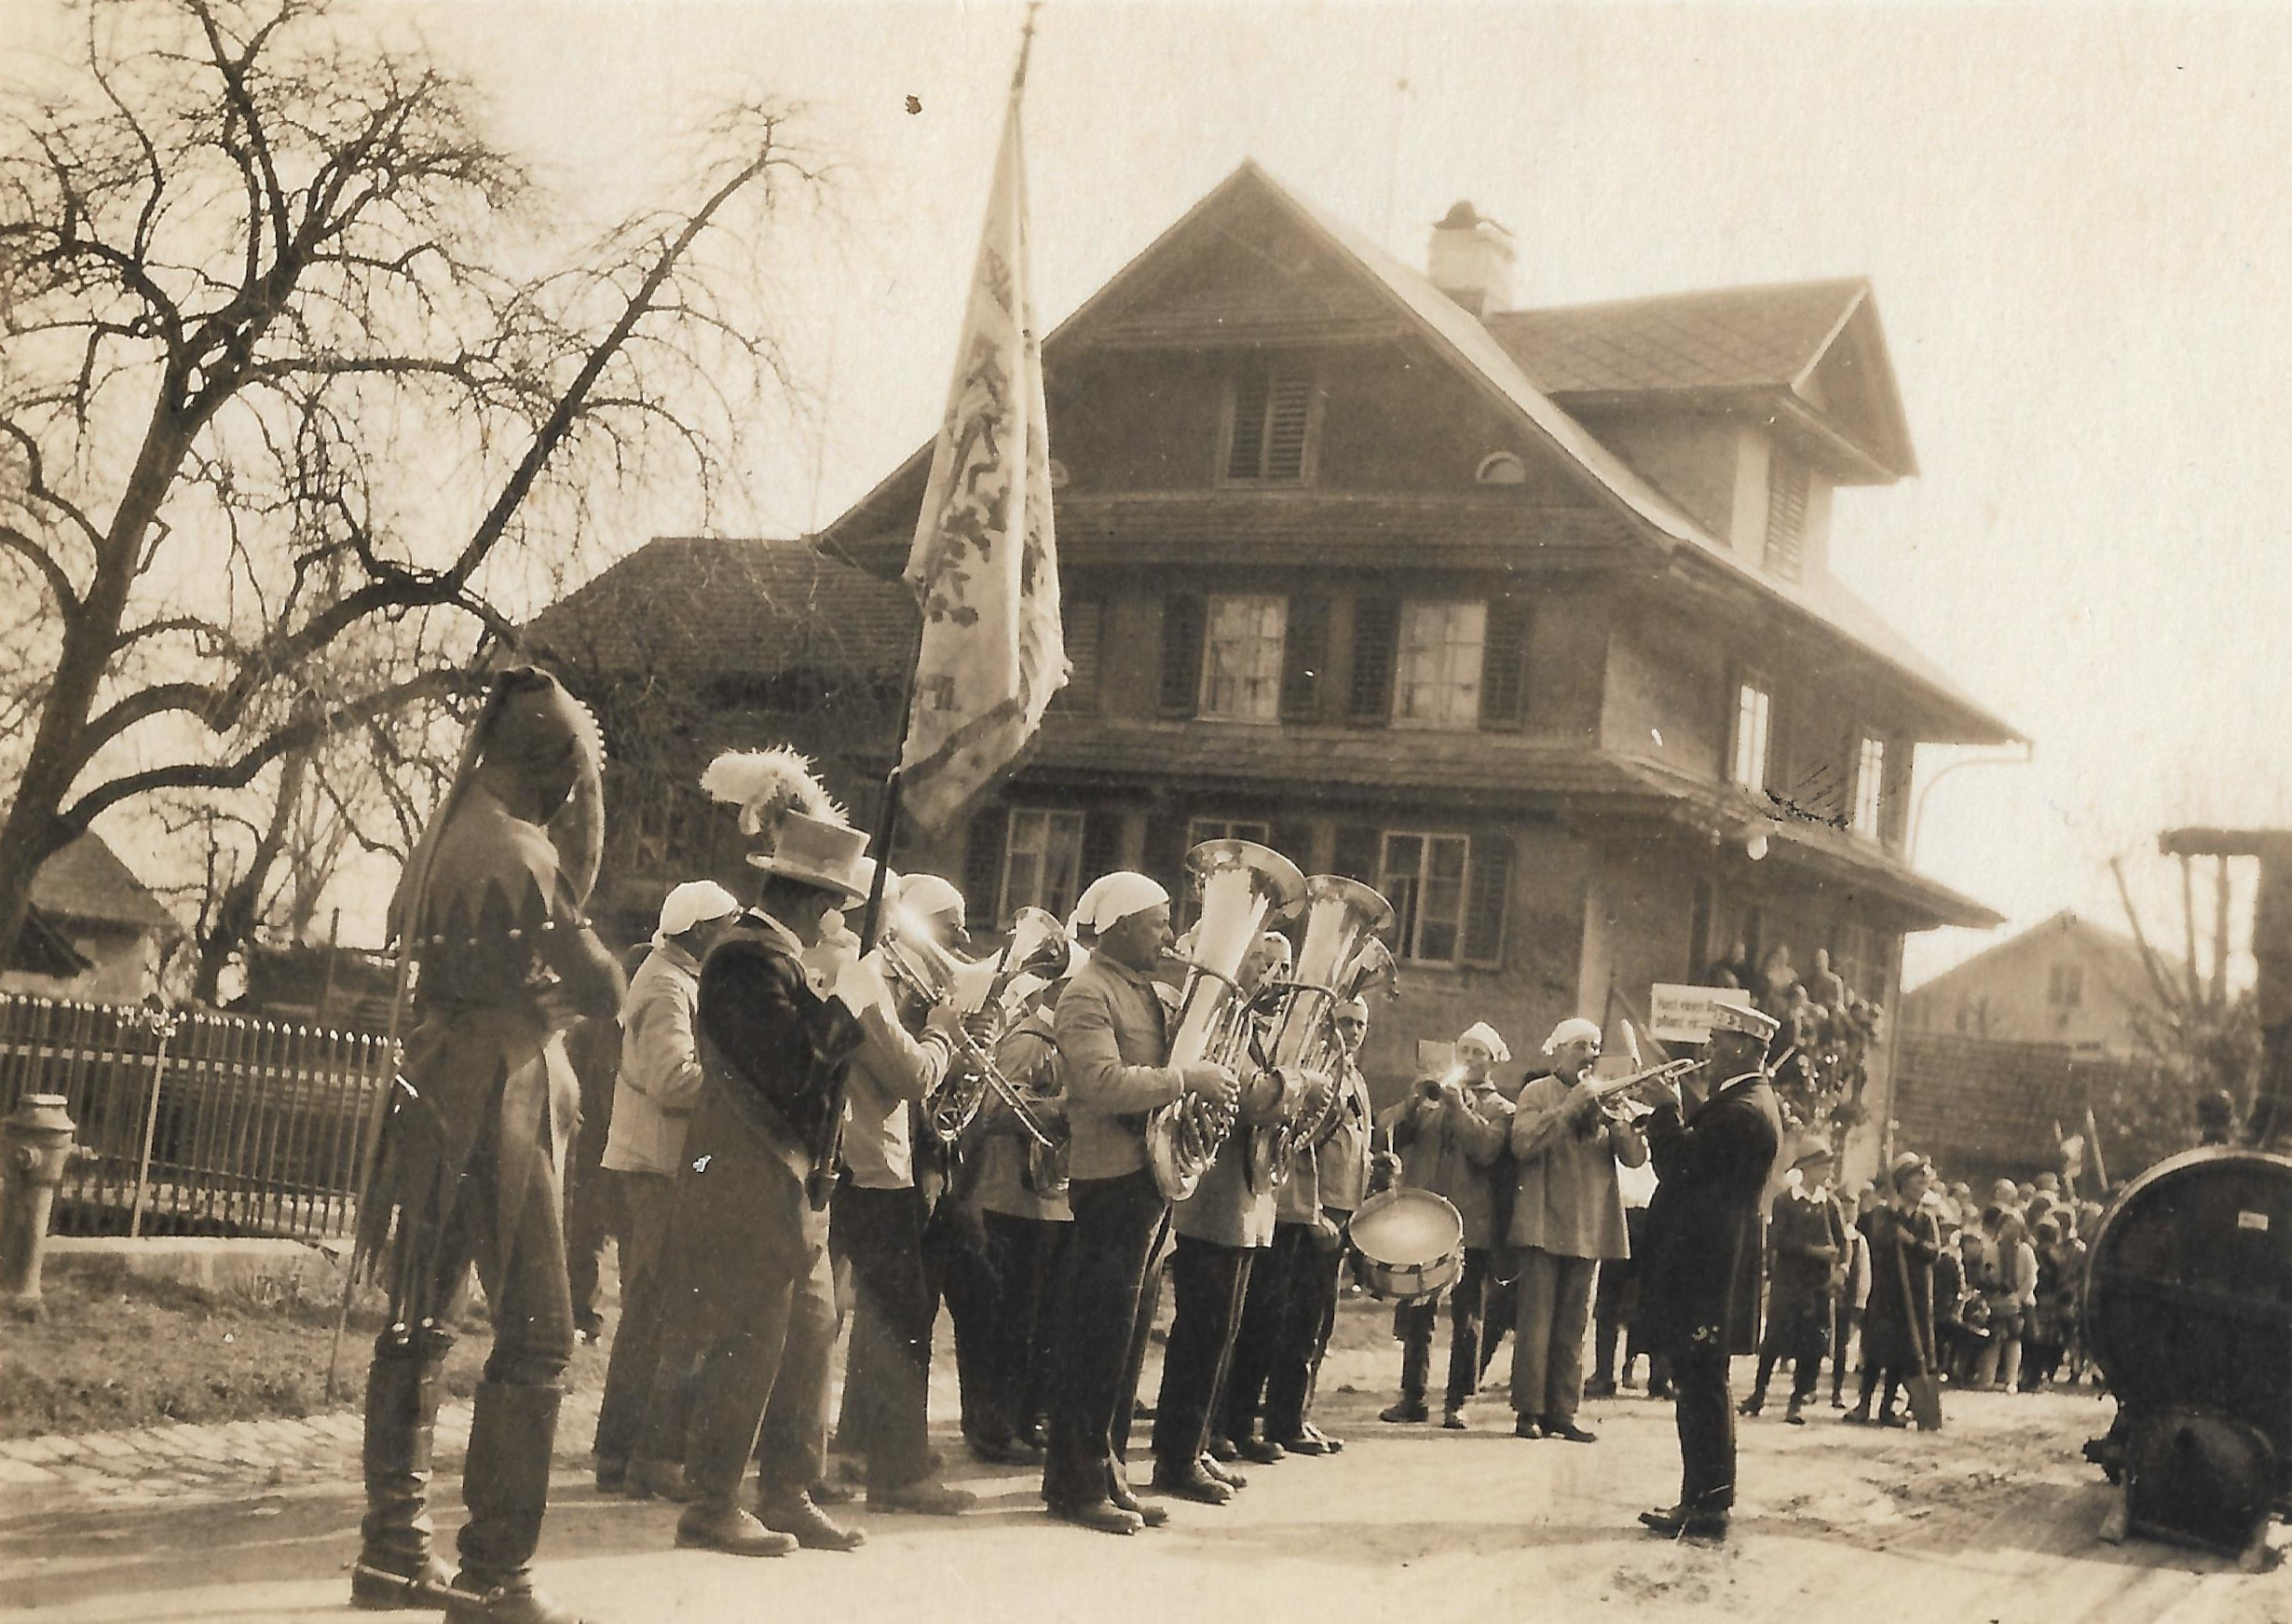
\includegraphics{./chap/1900-1925/Fasnacht-1920er-1.jpg}
        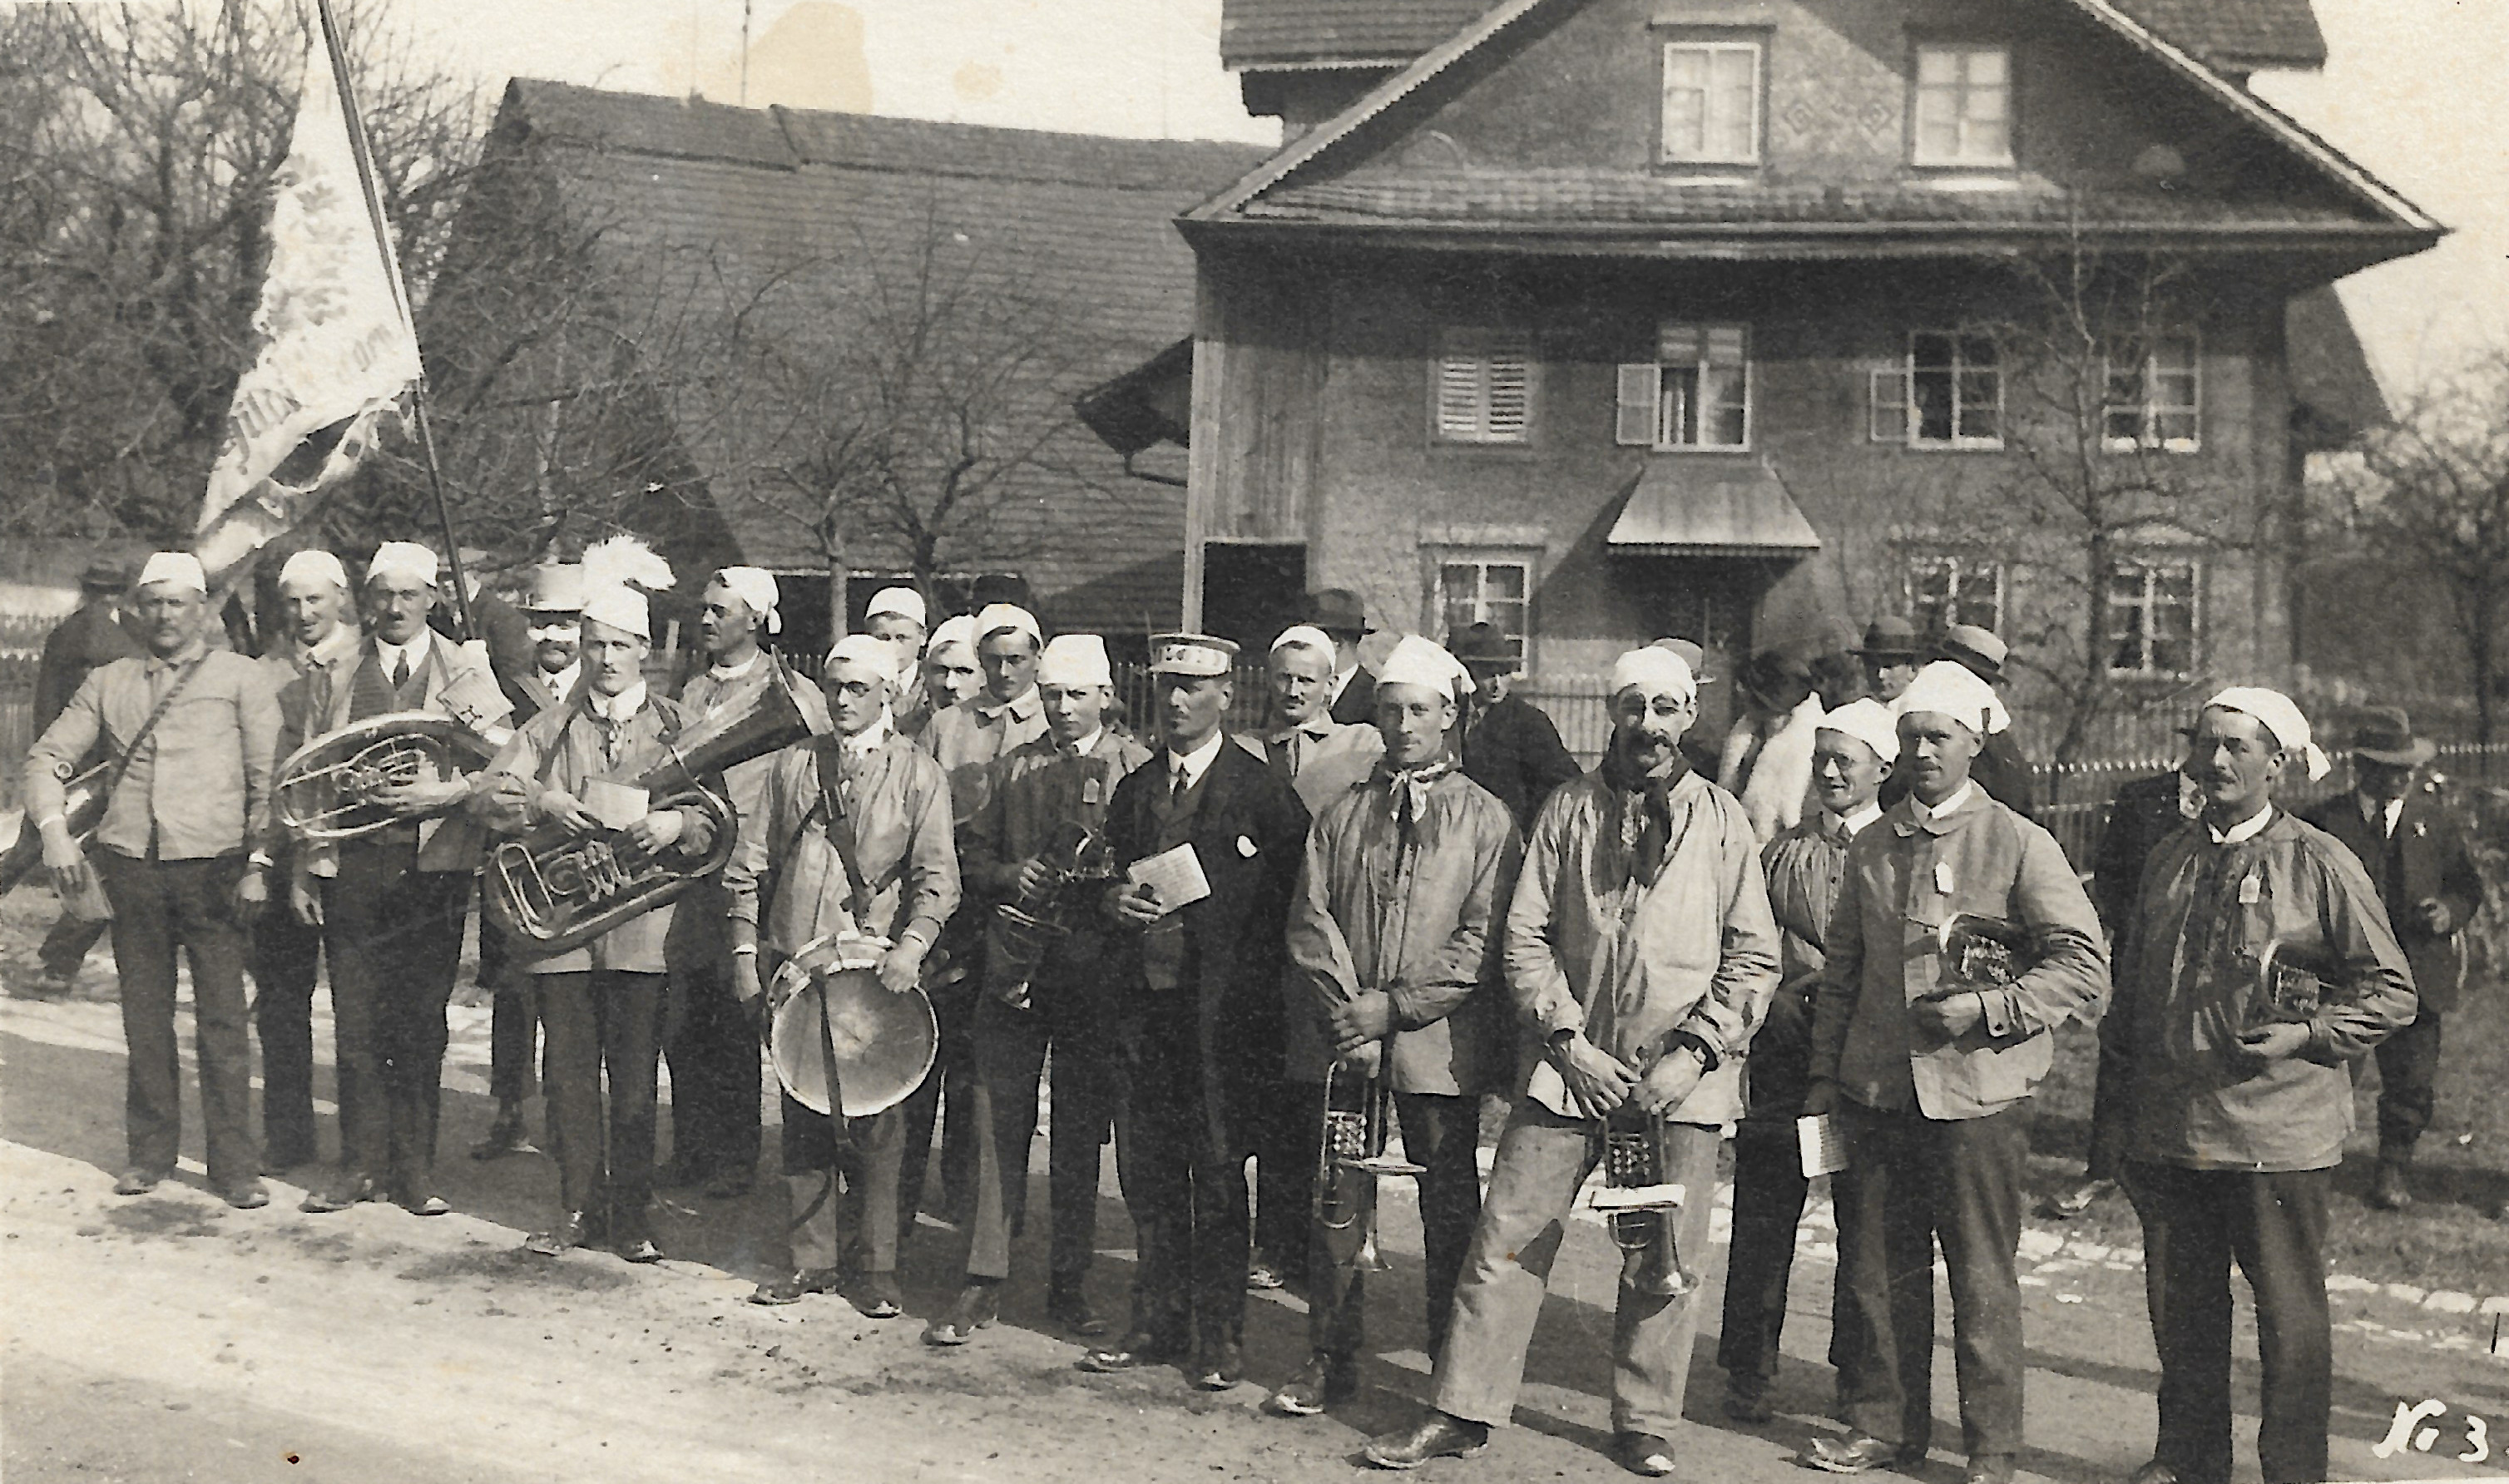
\includegraphics{./chap/1900-1925/Fasnacht-1920er-2.jpg}}
    \label{fig:mgh-fasnacht-1920}
    \caption{Fasnacht in den 1920ern}
\end{figure}

